\documentclass[11pt]{article}
\usepackage{geometry}
\geometry{letterpaper}
\documentclass{article}
\usepackage{rotating}
\usepackage{pdflscape}

\usepackage{graphicx}
\usepackage{amssymb}
\usepackage{float}
\usepackage{tabularx}
\usepackage{multicol}
\usepackage{rotating}
\usepackage{hyperref}
\hypersetup{
    colorlinks,
    citecolor=black,
    filecolor=blue,
    linkcolor=black,
    urlcolor=black
}

\begin{document}

\begin{titlepage}
	\newcommand{\HRule}{\rule{\linewidth}{0.2mm}}
	\begin{center}
	\textsc{\LARGE McMaster University}\\[1.5cm]

	\textsc{\Large HydroSwarm}\\[0.5cm]
	\textsc{\large Software \& Mechatronics Capstone}\\[0.5cm]

	\HRule\\[0.4cm]
		{\huge\bfseries Component Design}\\[0.4cm]
	\HRule\\[0.4cm]

	\begin{minipage}[t][][t]{0.5\textwidth}
		\begin{flushleft} \large
			\emph{Authors:}\\
			Victor Velechovsky - \textit{001305263}
			Amandeep Panesar - \textit{001431191}
			Nishanth Balamohan - \textit{001411319} \\
			Gabriel Potter - \textit{001429884} \\
			Taha Mian - \textit{001417172}
		\end{flushleft}
	\end{minipage}
	~
	\begin{minipage}[t][][t]{0.4\textwidth}
		\begin{flushright} \large
			\emph{Professor:} \\
			Dr. Alan Wassyng \\[0.4cm]
			\emph{Teaching Assistants:} \\
			Nicholas Annable \\
			Joshua Barkovic \\
			Spencer Deevy \\
			Viktor Smirnov
		\end{flushright}
	\end{minipage}\\[2cm]

	
\includegraphics[width=0.3\textwidth]{img/logo.png} \\
	{\large Last compiled on \today}
	\end{center}

\end{titlepage}

\tableofcontents
\listoffigures

\vfill
\begin{figure}[H]
   \centering
   \noindent\begin{tabularx}{\textwidth}{| >{\centering\arraybackslash}m{0.2\textwidth} | >{\centering\arraybackslash}m{0.2\textwidth} | >{\centering\arraybackslash}m{0.2\textwidth} | >{\centering\arraybackslash}m{0.285\textwidth} |}
   \hline
   \textbf{Date} & \textbf{Revision} & \textbf{Comments} & \textbf{Author(s)} \\ \hline
   Jan 4, 2019 & 1.0 & Document skeleton added & Victor Velechovsky \\ \hline
   Jan 8, 2019 & 1.1 & MID added & All authors \\ \hline
   Jan 9, 2019 & 1.2 & Some diagrams added & All authors \\ \hline
   Jan 10, 2019 & 1.3 & (Almost) final revision 0 & All authors \\ \hline
   Jan 18, 2019 & 1.4 & Final Revision 0 & All authors \\ \hline
   \end{tabularx}
   \caption{Revision History}
\end{figure}
\newpage
\section{Introduction}
\subsection{Purpose}
The purpose of this document is to outline the design of individual components that will be used in the HydroSwarm system. This document will also detail specifics about the HydroSwarm structure that is critical to its final implementation. The intended audience for this document is the internal team and other stakeholders who are concerned with the inner workings of the system. This document will serve as a guide during the development process and will help verify and validate design choices. It will also go undergo revision as the development of the system progresses. 
\subsection{Scope}
The scope of this document will cover the software design required to build the HydroSwarm system. It will cover modules such as: Area Coverage Algorithm, Server Communication, Data Storage, Insect Communication, Insect Motor Control, Insect Tracking/Locationing, and Insect Measurement Unit. 
\subsection{Project Overview}
HydroSwarm is a swarm of autonomous robotic boats meant to carry out measurements over large bodies of water. For our project, these boats will be measuring water temperature, but the idea can be expanded to any number of other quantifiable measurements. Central to our work will be two major components. First, a small motorized boat, attached with a water temperature sensor, as well as a control unit that allows it to communicate with and be controlled by a centralized control unit. Second, a software package that can control a large group (\hyperref[sec:definitions]{swarm}) of these boats, with an algorithm focused on producing reliable, accurate, and fast measurements.\\

Our swarm will aim to cover large areas more quickly and cost-effectively than traditional products. To test the applicability of our project, we will demo it on a small scale body of water, such as a swimming pool, as well as develop a simulation to hypothetically prove the efficacy of the system on a larger scale.\\

Our project will be conducted between Fall 2018 –- Winter 2019 for our Engineering Capstone project at McMaster University, under the guidance of Dr. Alan Wassyng. We have four Software Engineering students, and one Mechatronics Engineering student. \\ \\
\subsection{Naming Conventions and Terminology}
\label{sec:definitions}
The following terms and definitions will be used throughout this document:
\begin{itemize}
% Alphabetical order is highly preferred as it eases user navigation
\item \textbf{System}: The entire software and hardware package - including the boats,
boat hardware, control software, and server running the control software
\item \textbf{Swarm}: A large group of objects (in our case, motorized boats) that can communicate and perform acts as a group
\item \textbf{Insect}: A member of the swarm (in our case, a single motorized boat)
\item \textbf{Simulation}: The simulation will be used for demo purposes, mainly to show that
the system is valid with a large number of insects.
\item \textbf{Researcher}: A user that is interested in the data that is returned from the survey.
\item \textbf{System Administrator}: A user that controls the parameters of the \hyperref[sec:definitions]{\textbf{swarm}}.
\item \textbf{G.P.S.}: Global Locationing System
\item \textbf{Coverage area}: The area in which the insects are confined. This defines that space that the user wants to track and measure.
\item \textbf{API}: Application Programming Interface
\end{itemize}

\section{Subsystems}
The system will be broken down into the following subsystems:

\begin{itemize}
\item \textbf{Simulation}
\item \textbf{Insect Tracking/Positioning}
\item \textbf{Insect Motor Control}
\item \textbf{Insect Measurement Sensors}
\item \textbf{Server Communication Interface}
\item \textbf{Insect Communication Interface}
\item \textbf{User Interface}
\item \textbf{Area Coverage Algorithm}
\item \textbf{Data Storage}

\end{itemize}

\begin{figure}[H]
   \centering
   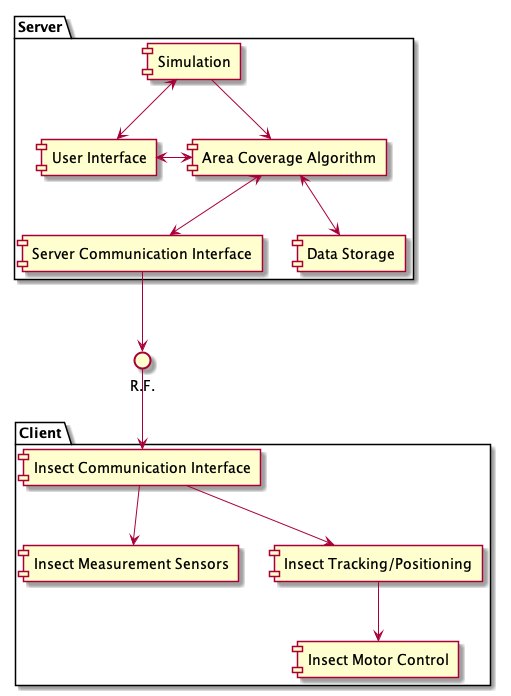
\includegraphics[width=0.8\textwidth]{diagram/component-diagram.png}
   \caption{Subsystem Breakdown}
   \label{fig:sub}
\end{figure}

\section{Detailed Class Diagram}
The Detailed Class Diagram is shown in Figure \ref{fig:dcd}, found in the Appendix.

\section{Likely Changes}
Development of Hydroswarm is still in its early stages, and thus there are a number of design decisions that
are likely to change:

\begin{itemize}
    \item \textbf{Insect positioning system}: The insect positioning system may end up being swapped for a different
    system that works based on G.P.S., Computer Vision tracking, Ultra-wide-band triangulation, or some other approach
    \item \textbf{Number of demo insects}: The number of insects used in the demo are currently set at three (one for
    the initial demo) but this may change based on financial or time constraints
    \item \textbf{Area Coverage Algorithm}: The implementation of the area coverage algorithm is still not entirely
    decided and may be overhauled if a more efficient or effective algorithm is invented
    \item \textbf{Insect Micro-controller}: The insects are currently using an Arduino to handle processing, I/O, and
    communication. This may change in the future, if a more power-efficient or cost-effective chip is found.
    \item \textbf{Boats vs. Cars}: Though our project is currently aimed at using boats to measurement temperature in
    water, if we run into technical difficulties, we may have to switch to cars that make measurements on dry land
    instead.
    \item \textbf{Communication API}: Throughout development the API through which different components communicate
    with one another may be tweaked in order to better facilitate system performance
\end{itemize}

\section{Module Guide}
\subsection{Server Components}
\subsubsection{Area Coverage Algorithm}
\textbf{Responsibilities} \\
The algorithm decides which locations each insect should travel to, in order to
completely cover the coverage area quickly. After each measurement, an insect will request
a new location to move to. The algorithm will calculate this value, and pass it on to the
insect so that it can begin travelling there. \\

\textbf{Secrets} \\
The decision making process of producing new locations for insects to move to. \\

\textbf{MID}

\begin{itemize}
    \item \textbf{public method setMeasurement} - double temperature, Insect i, Location p \\ returns: void \\ description: Sets a measurement at a given location
    \item \textbf{public method nextTarget} - Insect i \\ returns: \textit{Location} \\ description: Returns the next Location that Insect i should move to.
    \item \textbf{private method withinBoundary} - Location p \\ returns: \textit{boolean} \\ description: Determines whether the location
    p is in the predefined coverage area
    \item \textbf{private member coverageArea} - Region
    \item \textbf{private member numInsects} - Int
    \item \textbf{private member measurements - Measurement []} \\ description: Describes the history of all measurements that the insects have made.
    \item \textbf{private member currentLocation - Map$<$Insect, Location$>$} \\ description: Stores the current location of each insect
    \item \textbf{private member disabledInsects - Insect []} \\ description: Stores a list of insects that have been disabled or have encountered mechanical problems
\end{itemize}

\subsubsection{Server Communication}
\textbf{Responsibilities} \\
The server communication subsystem is responsible for communicating important information from the server to the insect. In addition, data will also be received from the insect which might contain information such as Location, temperature, and velocity. The data transmitted to the insect will
also follow a similar structure and include data such as desired speed and Location. The hardware components involved in the interaction will include a micro-controller and RF transceiver which has the ability to send and receive data. \\
\newline
\textbf{Secrets : } The channel and address the insects communicate on, along with the variables sent between the server and insects respectively. \\
\newline
\textbf{MID:}
\begin{itemize}
    \item \textbf{public member transmitNewLocation - Map$<$Insect, Location$>$} \\ description: sends target coordinates for specified insect
    \item \textbf{private member confirmRequest - Insect id}
    \\returns: \textit{boolean}
    \\description: sends target coordinates for specified insect id
    \item \textbf{public member receiveLocation - Insect id}
    \\ returns: \textit{Map$<$Insect, Location$>$} \\ description: request current Location of specified insect id 
    \item \textbf{public member receiveSensorData - Insect id} \\
    returns: \textit{Temperature} \\ 
    description: requests current Temperature at Insect id 
    
\end{itemize}
\subsubsection{Data Storage}
\textbf{Responsibilities}
The data storage subsystem is responsible for storing all data collected by each insect during the survey. Also data storage is responsible for querying data. Data storage will be able to add information based on a survey and all data collected by each insect and the location of where the data was collected. Data storage will interact with a document store database. Each survey will be its own data object, with details of the survey added as the survey progresses.
\\\\
\textbf{MID}
\begin{itemize}
    \item \textbf{public method createSurvey - Survey S} \\
    returns \textit{void} \\
    Description: Creates a new survey object in Database
    \item \textbf{public method insertSurveyData - Data D, String ID} \\
    returns \textit{void} \\ 
    Description: Inserts data into survey object in database given a survey ID.
    \item \textbf{public method getSurvey - String ID } \\
    returns \textit{Survey} \\
    Description: Gets all information about a certain survey given an ID
    \item \textbf{ public method  createSimulation - Simulation Sim} \\
    returns \textit{void} \\
    Description: Creates a simulation object in the database
    \item \textbf{public method insertSimData - Data D, String ID} \\
    returns \textit{void} \\
    Description: inserts data into a simulation object in database given a simulation ID
    \item \textbf{public method getSimulation - String ID} \\
    returns \textit{Simulation} \\
    Description: Takes a string parameter which is the ID of a simulation object, and searches database for matching Simulation object, and returns it.
\end{itemize}
\subsubsection{Simulation}
\textbf{Responsibilities}
The simulation system will be responsible for allowing user to run a simulation of the survey. Simulation system uses the area coverage system to mimic an actual survey. \\
\textbf{MID}
\begin{itemize}
    \item \textbf{public method genSimulation - Region R, Int numInsects } \\ 
    returns \textit{void} \\
    Description: Creates a simulation object, in the data storage, and simulates a survey using area coverage system.
    \item \textbf{public method stopSimulation} \\
    returns \textit{void} \\
    Description: stops simulation if its running
    \item \textbf{private member ID - String} \\
    Description: ID for a simulation
\end{itemize}
\subsubsection{User Interface}
\textbf{Responsibilities}\\
The User Interface is responsible for allowing the user to interact with the swarm during operation as well as running the simulation. The User Interface will be able to initialize the surveying process and display the measurements made by the insects. It will also have the ability to override any insect controls in the case of a malfunctioning insect. The U.I. also has the responsibility of displaying the simulation to the user, allowing them to change any parameters to run the simulation.\\
\newline
\textbf{Secrets: }Implementation details of the interface, abstract all the unnecessary information to the user. The UI should only present the important data that the user needs to see. \\

\textbf{MID}
\begin{itemize}
    \item \textbf{public method goToMain -- ActionEvent e}\\ returns: void \\ Description: Goes to the main page.
    \item \textbf{public method goToSurvey -- ActionEvent e}\\ returns: void \\ Description: Goes to the survey page.
    \item \textbf{public method goToSimulation -- ActionEvent e}\\ returns: void \\ Description: Goes to the simulation page.
    \item \textbf{private member systemState}\\ Description: Contains the states NONE, SIMULATION and SURVEY.
    \item \textbf{private method setSystemState -- systemState}\\ returns: void \\ Sets the system state according to the actions the user selected.
    \item \textbf{public method startSimulation -- Region P, Int num, Action Event e}\\ returns: void \\ Description: Takes the parameters that the user inputs and calls the necesary functions from the Area Coverage Algorithm to run the simulation. Sets systemState to SIMULATION.
    \item \textbf{public method endSimulation -- ActionEvent e}\\ returns: void \\ Description: Stop the simulation. Sets the systemState to NONE.
    \item \textbf{public method createChart -- State systemState}\\ returns: void \\ Description: While the simulation is running, this function will call the necessary functions to visualize the paths of the insects. Depending on the state of system the visualizations will display different data.
    \item \textbf{public method startSurvey -- Region P, Int num, Action Event e}\\ returns: void \\ Description: While the survey is in progress this method visualized the data that is returned by the insects. Sets systemState to SURVEY.
    \item \textbf{public method endSurvey -- ActionEvent e}\\ returns: void \\ Description: Stops the current survey. Sets systemState to NONE.
\end{itemize}

\subsection{Insect Components}
\subsubsection{Insect Communication}
\textbf{Responsibilities}\\
The insect communication subsystem is responsible for communicating vital information from the insect to the server. The data  transmitted will include sensor data, GPS coordinates,and accelerometer output. The data received from the server will include information such as speed and direction based on algorithm output. The hardware components interacting with this subsystem will include a micro-controller and RF transceiver which will have the ability to send and receive data The input will include data that will be sent to the server such as temperature logged, current Location, id, and velocity. The output will be the data received by the server such as desired velocity and Location. \\
\newline
\textbf{Secrets : } The channel and address the server communicates on, along with the variables sent between the server and insect respectively. \\
\newline
\textbf{MID:}
\begin{itemize}
    \item \textbf{public member receiveNewLocation - null} \\ description: receives target coordinates for specified insect
    \item \textbf{public member transmitLocation - Map$<$Insect, Location$>$}
    \item \textbf{private member transmitConfirmation - Insect id}
    \\ description: Sends confirmation that request has been received by insect id
    \item \textbf{public member transmitSensorData - Insect id, Temperature} \\
    description: sends current Temperature with Insect id 
    
\end{itemize}

\subsubsection{Insect Motor Control}
\textbf{Responsibilities}\\
The motor control subsystem will provide a means for controlling the velocity of each insect.
Each boat in the swarm will have this subsystem which will be responsible for interpreting the
desired speed and direction data received from the communications and Locationing subsystems
and enacting those instructions by sending the appropriate signals to the motors present on each
boat. Each boat has left and right motors which can be controlled separately to achieve speed and direction changes to a boat's velocity. \\
\newline
\textbf{Secrets: } The motor control signals, i.e. the ports and voltages required for controlling each motor. \\
\newline
\textbf{MID:}
\begin{itemize}
    \item \textbf{public method setMotorState - motorState} \\ description: Called by the Locationing subsystem to change the state of the motors. The caller passes a motorState structure (defined below).
    \item \textbf{private member motorState} \\ description: Contains variables outputSpeed, state, and argPtr (defined below). \\
    masterSpeed: The percentage of maximum motor output (0-1). \\
    state: The desired motor state. \\
    argPtr: Allows extra necessary arguments to easily be passed to the motor control module, i.e. the ratio argument for the method below.
    \item \textbf{private method steerLeft - float ratio} \\ 
    description: Corresponds to state STEERLEFT. Ratio is the degree to which the left motor is underpowered in comparision to the right motor (controls the sharpness of the turn). Note that ratio can be negative; this would cause the left motor to operate in reverse.
    \item \textbf{private method steerRight - float ratio} \\ 
    description: Corresponds to state STEERRIGHT. Ratio is the degree to which the right motor is underpowered in comparision to the left motor (controls the sharpness of the turn). Note that ratio can be negative, this would cause the right motor to operate in reverse.
    \item \textbf{private method forward} \\ 
    description: Corresponds to state FORWARD. Puts both motors in forward rotation at power defined by outputSpeed.
    \item \textbf{private method reverse} \\ 
    description: Corresponds to state REVERSE. Puts both motors in reverse rotation at power defined by outputSpeed.
    \item \textbf{private method shutdown} \\ 
    description: Corresponds to state SHUTDOWN. Cuts power to both motors.
\end{itemize}

\subsubsection{Insect Tracking/Locationing}
\textbf{Responsibilities}\\
The insect tracking and Locationing subsystem is responsible for determining the Location of each
individual insect within the area of coverage, and ensuring that the boat is adhering to the desired
velocity specified by the area coverage algorithm. Therefore each insect/boat will be equipped with
this subsystem. Hardware components of this subsystem include the micro-controller and GPS
module. This subsystem will interact with the communications subsystem and the motor control subsystem. It will send GPS coordinates and velocity to the communications subsystem, and it
will calculate slight adjustments to the boat velocity and send these updates to the motor control
subsystem. \\
\newline
\textbf{Secrets: } Implementation details of the interface to the GPS and accelerometer chips. \\
\newline
\textbf{MID:}
\begin{itemize}
    \item \textbf{public method getLocation} \\ description: Returns current Location of the boat.
    \item \textbf{public method getAcceleration} \\ description: Returns accelerometer data.
    \item \textbf{public member desiredLocation} \\ description: This is the desired Location of the boat as specified by the area coverage algorithm.
    \item \textbf{private method getNewMotorState} \\ description: Uses current Location and speed data along with desired Location data to determine if the motor state needs to be adjusted.
\end{itemize}
\begin{figure}[H]
   \centering
   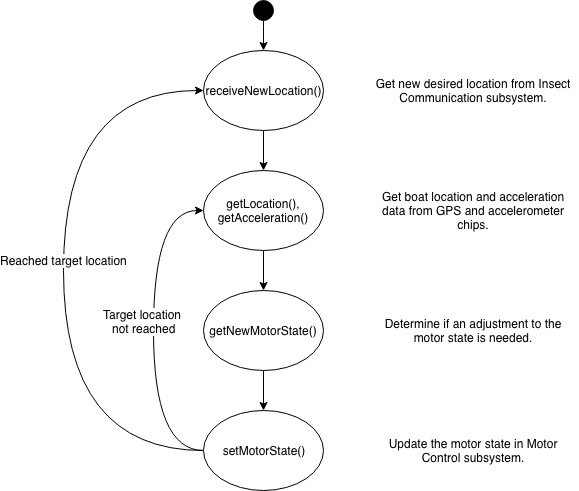
\includegraphics[width=0.8\textwidth]{diagram/location_ctrl_fsm.png}
   \caption{Location Control FSM}
\end{figure}

\subsubsection{Insect Measurement Unit}
\textbf{Responsibilities}\\
The insect measurement unit will be the component that is responsible for the temperature readings from the sensor. The sensor will make measurements which will be called periodically. \\
\newline
\textbf{Secrets: }The communication channel and the measurement data that is sent to the server. \\
\textbf{MID:}
\begin{itemize}
    \item \textbf{public method getTemperature} \\ Description: This method will return the current temperature reading of the sensor.
\end{itemize}

\section{Communication Protocols}
\subsection{Algorithm/User Interface}
The server and user interface will both be programmed in C++ and will communicate through C++ API calls.
\subsection{Algorithm/Server Communication API}
The server and user interface will both be programmed in C++ and will communicate through C++ API calls.
\subsection{Server Communication API/Insect Communication API}
The server will communicate with insects through Radio Frequency. Each node will have an RF transciever that can send & receive
data on a particular channel (which will be set manually for each insect).
\subsection{Insect Communication API/Other Insect Modules}
Here, 'Other Insect Modules' refers to:
\begin{itemize}
    \item Insect Motor Control
    \item Insect Tracking/Location
    \item Insect Measurement Unit
\end{itemize}

All of these modules will be able to call each others public-facing functions as they will be running on a shared codebase.
\subsection{Algorithm/Data Storage}
The Database will be accessed by the algorithm through the use of ODBC (Open Database Connectivity).

\section{Scheduling}
While it is difficult at this time to determine precisely defined timing constraints, there are several timing and scheduling concerns which are necessary for the most optimal operation of the system. These are outlined in the subsections below.

\subsection{Algorithm/Server Timing Constraints}
To facilitate the smoothest possible operation of the swarm, each insect should know its next destination before it reaches its current destination. This ensures that time is not wasted by the insect in waiting for instructions at each measurement point. The system should satisfy the sequence diagram below.
\begin{figure}[H]
   \centering
   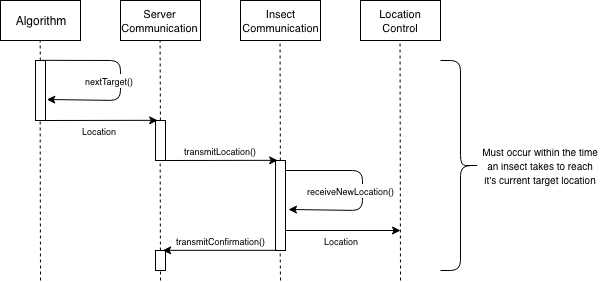
\includegraphics[width=1\textwidth]{diagram/next_target_sequence.png}
   \caption{Sequence diagram for determining next location}
\end{figure}
While this scheduling constraint should be relatively easy to meet for a small number of insects, when the swarm begins to grow it may be necessary to prioritize these calculations based on which insect is closest to its current target location.

\subsection{Location Control System}
Due to the presence of drift and other anomalies found in lakes, oceans, etc. that will affect the trajectory of each insect, each insect should be able to correct its path as necessary as it makes its way toward the target location. This means each insect must update its current location at a high enough frequency and in a timely enough manner for the control system to work properly and to prevent the insect from drifting too far from its intended route.
\begin{figure}[H]
   \centering
   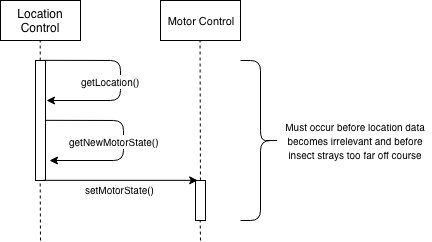
\includegraphics[width=0.7\textwidth]{diagram/location_control_sequence.png}
   \caption{Sequence diagram for adjusting insect path}
\end{figure}

\subsection{Hardware Design Notes}
\subsubsection{Motor Control}
The motors on-board the insect are paired with a 3rd party remote controller out of the box, and needs to be changed to allow the server to move the insects. The server will most likely use RF transceivers to send commands to the insects, but a hardware controller is required to interface with the motors. This is where the L239D integrated circuit (IC) comes into play, since it allows any arbitrary microcontoller to be able to interface with the motors bidirectionally. In addition to interfacing with both motors, the time it takes to turn on each individual motor is almost instantaneous. The result of an instantaneous motor control allow the swarm of insects to adapt and change very quickly. The design or wiring schematic of the L239D is given below. 

\begin{figure}[H]
   \centering
   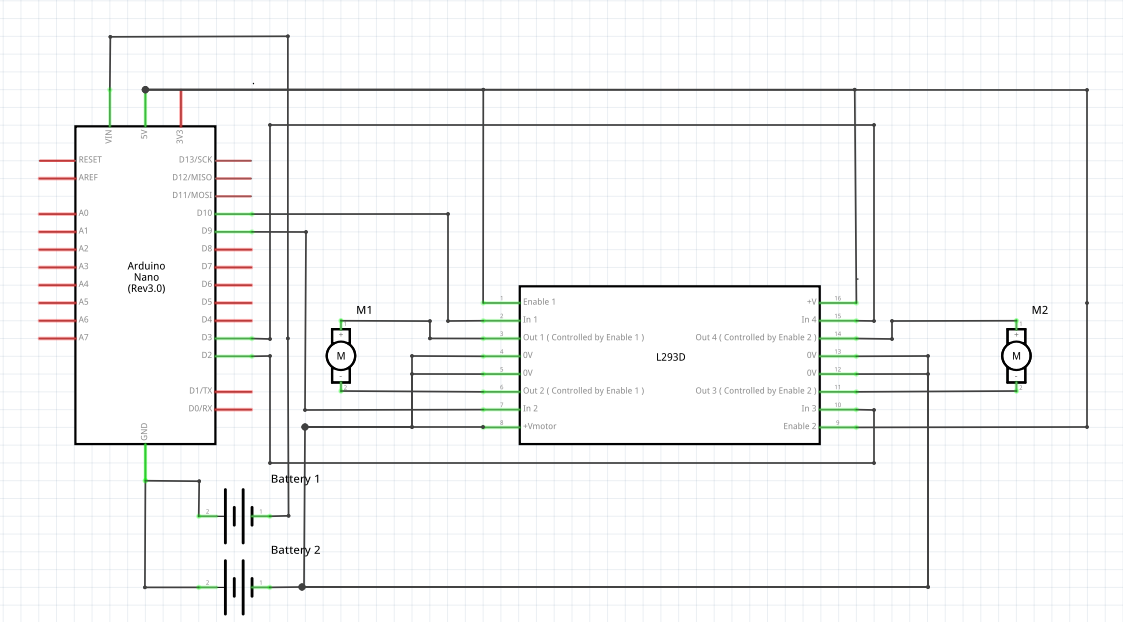
\includegraphics[width=\textwidth]{img/MotorWiringDiagram.png}
   \caption{Wiring Diagram for Motor Control}
\end{figure}

\subsubsection{RF Control}
Communication between the insects and the server must be quick and the range must be limitless to be able to scale the system. The nRF24L01 allows the server to do both, even though the maximum range is described as 20 feet. The range is however limitless when using the associated library since the transceivers can be setup in a mesh network. In addition, RF is also easier to prototype in regards to Arduino and has fairly quick response time through some testing the group has done. The figure below contains the wiring diagram for the nRF24L01 transceiver.  
\begin{figure}[H]
   \centering
   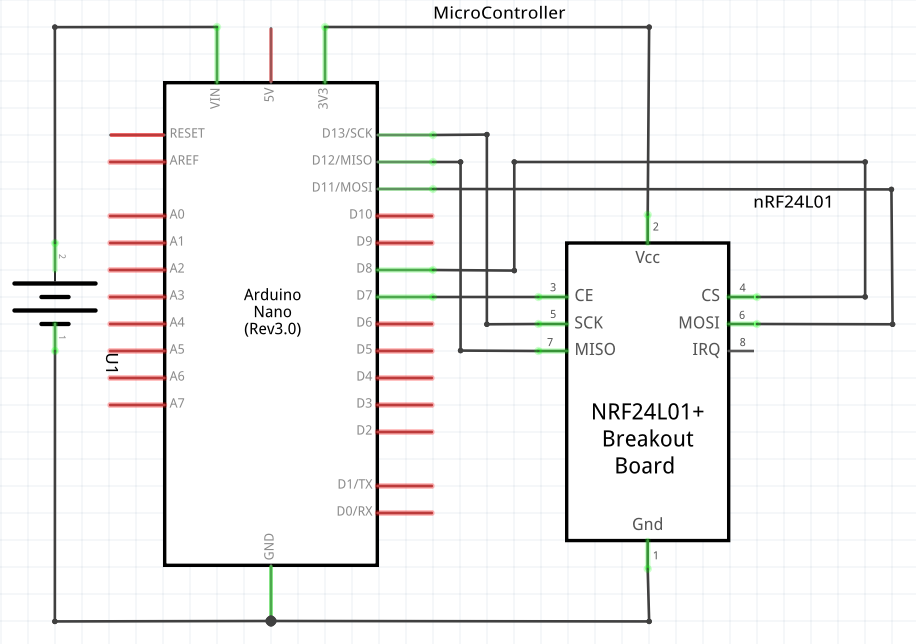
\includegraphics[width=\textwidth]{img/nRFWiringDiagram.png}
   \caption{Wiring Diagram for nRF24L01 Transceiver}
\end{figure}

\subsubsection{Gyroscope and Accelerometer Design}
One of the requirements for the system is for the algorithm to know where the boats are and how fast they are traveling. The Gyroscope allows the insect and server to measure its current orientation. The Accelerometer helps with the second part of the requirement and lets the algorithm know the velocity of the individual insect. The combination of both outputs from the Gyroscope and Accelerometer lets the system know the approximate location and even remaining time for the current survey in progress. However, both sensors must be compact and power efficient to be able to achieve maximum efficiency, thus the MPU6050 sensor was chosen. This integrated circuit is capable of a total of six degrees of freedom and is more power efficient than two individual Accelerometer and Gyroscope sensors respectively. In addition, the polling rate is around 50 samples per second which allows quick response to the server if needed. The schematic wiring diagram for the MPU 6050 is shown in the figure below.  
\begin{figure}[H]
   \centering
   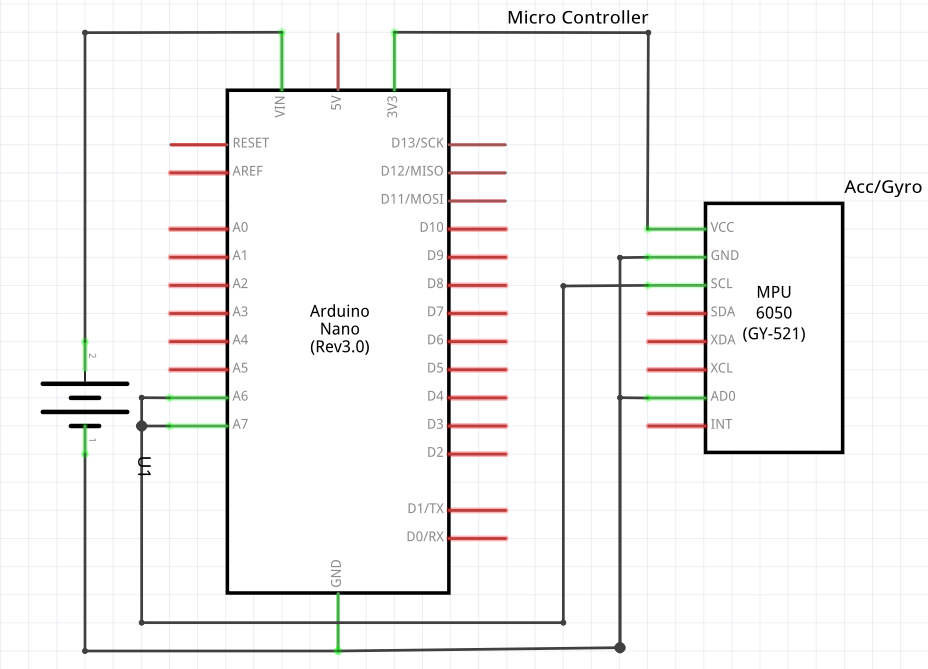
\includegraphics[width=\textwidth]{img/MPU6050Wiring.png}
   \caption{Wiring Diagram for MPU6050 Sensor}
\end{figure}

\section{Module-Requirement Traceability Matrix}

The following definitions highlight the acronyms used for each component in the traceability matrices:
\begin{itemize}
    \item \textbf{ACA}: Area Coverage Algorithm
    \item \textbf{SC}: Server Communication
    \item \textbf{DS}: Data Storage
    \item \textbf{SIM}: Simulation
    \item \textbf{UI}: User Interface
    \item \textbf{IC}: Insect Communication
    \item \textbf{IMC}: Insect Motor Control
    \item \textbf{ITL}: Insect Tracking/Location
    \item \textbf{IMU}: Insect Measurement Unit
\end{itemize}

\begin{table}[H]
\centering
\caption{Module-Functional Requirement Traceability Matrix}
\label{my-label}
\begin{tabular}{|l|l|l|l|l|l|l|l|l|l|}
\hline
Requirement ID & ACA & SC & DS & SIM & UI & IC & IMC & ITL & IMU \\ \hline
F1             &     &    &    &     &    &    &     &     & X   \\ \hline
F2             &     &    &    &     &    &  X &     &  X  &     \\ \hline
F3             &     &    &    &     &    &  X &  X  &  X  & X   \\ \hline
F4             &  X  &  X & X  &     & X  &    &     &     &     \\ \hline
F5             &     &    &    &     &    &    &  X  &  X  &     \\ \hline
F6             &  X  &    &    &     &    &    &  X  &  X  &     \\ \hline
F7             &  X  & X  &    &     &    &    &  X  &  X  &     \\ \hline
F8             &  X  &    &    &     &    &  X &  X  &     &     \\ \hline
F9             &     & X  &    &     &    &    &     &  X  &     \\ \hline
F10            &  X  & X  &    &     &    &  X &  X  &  X  & X   \\ \hline
\end{tabular}
\end{table}

\begin{table}[H]
\centering
\caption{Module Non-Functional Requirement Traceability Matrix}
\label{my-label}
\begin{tabular}{|l|l|l|l|l|l|l|l|l|l|}
\hline
Requirement ID  & ACA & SC & DS & SIM & UI & IC & IMC & ITL & IMU  \\ \hline
NF1             &     &    &    &     &  X &    &     &     &      \\ \hline
NF2             &     &    &    &     &  X &    &     &     &      \\ \hline
NF3             &     &  X &  X &     &  X &    &     &     &  X   \\ \hline
NF4             &     &  X &  X &     &    &    &     &     &  X   \\ \hline
NF5             &  X  &    &    &  X  &    &    &     &     &      \\ \hline
NF6             &     &  X &    &     &    &    &     &     &      \\ \hline
NF7             &     &  X &    &     &    &  X &     &     &      \\ \hline
NF8             &     &    &    &     &    &    &     &     &      \\ \hline
NF9             &     &  X &  X &     &    &  X &     &     &      \\ \hline
NF10            &     &    &    &     &  X &    &     &     &      \\ \hline
NF11            &     &    &    &     &    &    &     &     &      \\ \hline
NF12            &     &    &    &     &    &    &  X  &     &      \\ \hline
NF13            &     &    &    &     &    &    &     &     &      \\ \hline
\end{tabular}
\end{table}
\newpage
\section{Appendix}
\subsection{Class Diagram}
The Class Diagram gives an overview of the layout of the system.
\begin{sidewaysfigure}[ht]
   \centering
   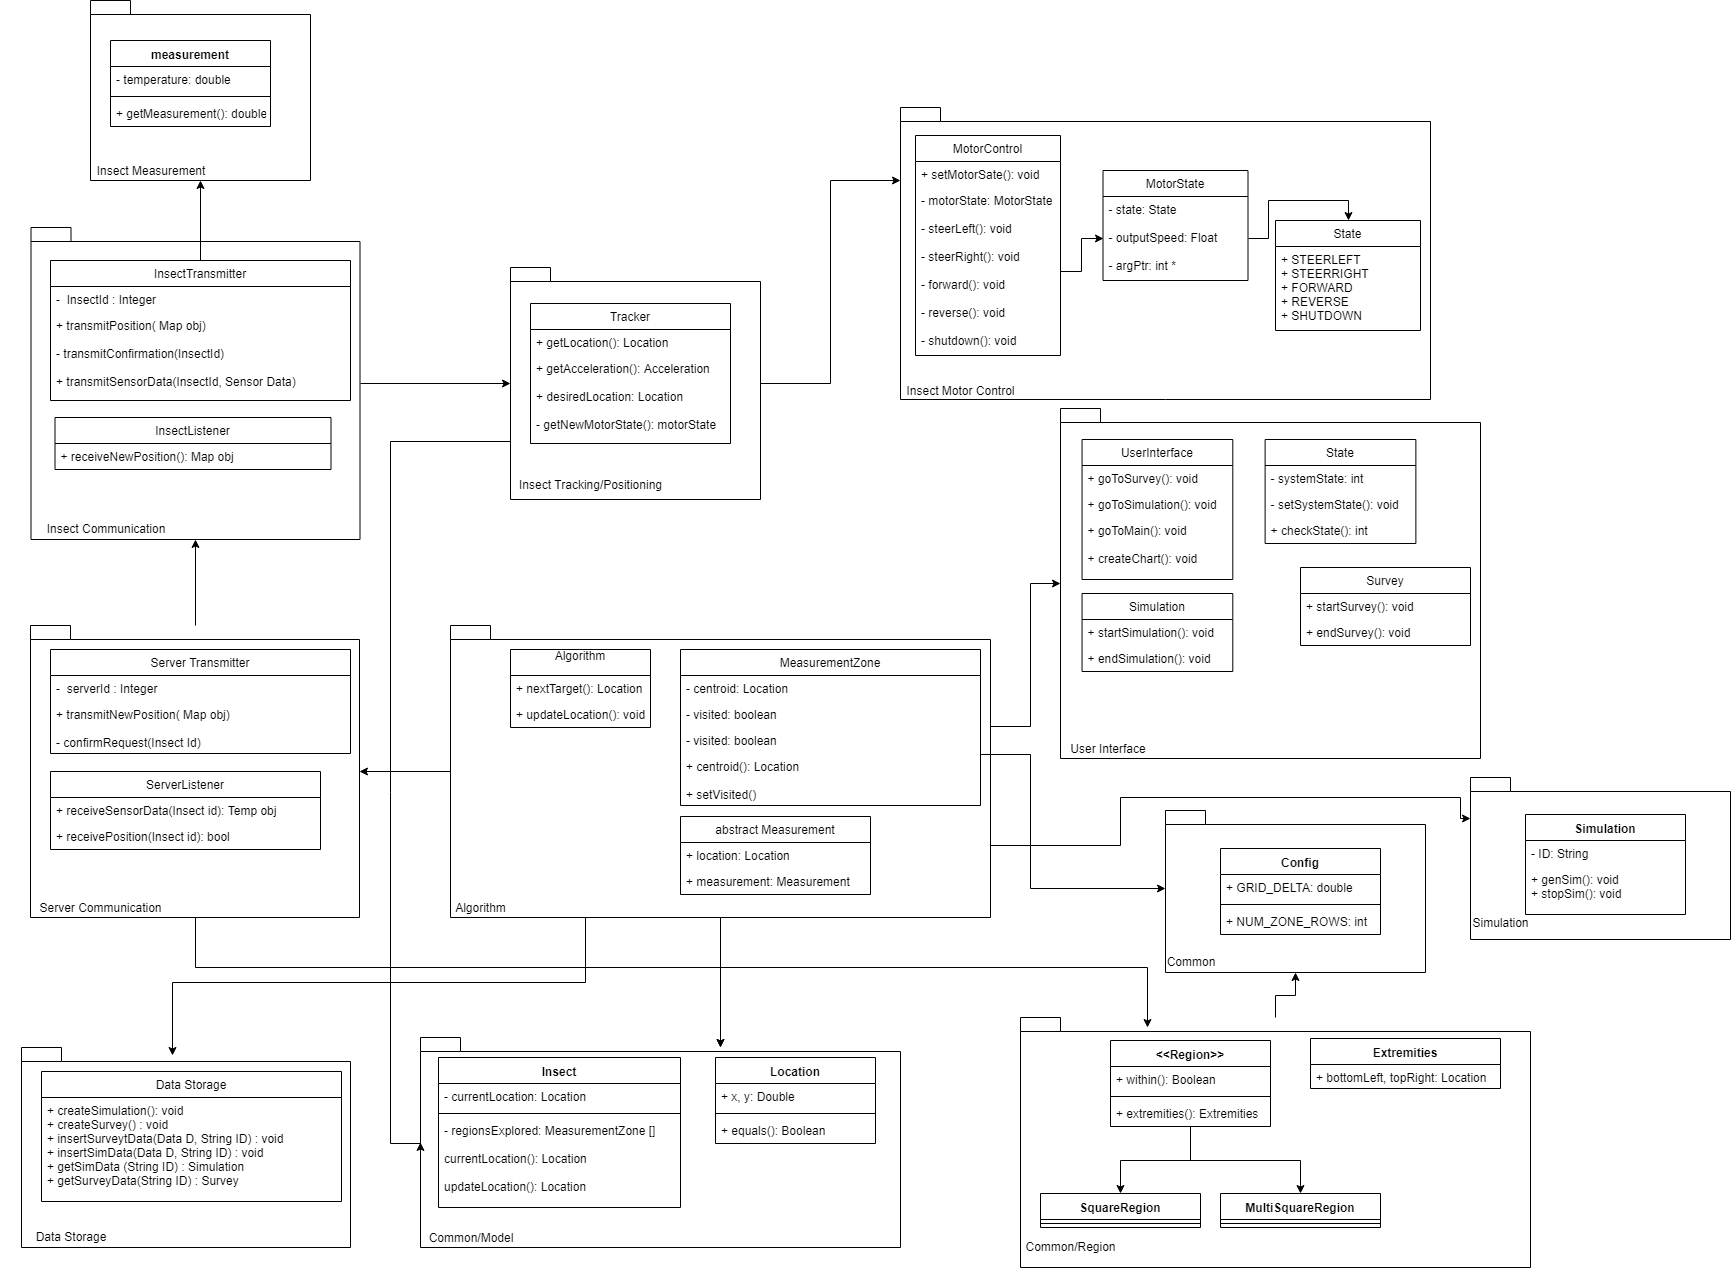
\includegraphics[width=\textwidth]{diagram/class_diagram_final2.png} % requires the graphicx package
   \caption{Detailed Class Diagram}
   \label{fig:dcd}
\end{sidewaysfigure}

\end{document}
